\documentclass[conference]{IEEEtran}
\IEEEoverridecommandlockouts

\usepackage{cite}
\usepackage{amsmath,amssymb,amsfonts}
\usepackage{algorithmic}
\usepackage{graphicx}
\usepackage{textcomp}
\usepackage{xcolor}
\usepackage{hyperref}
\usepackage{booktabs}
\usepackage{array}
\usepackage{multirow}
\usepackage{tikz}
\usepackage{pgfplots}
\pgfplotsset{compat=1.18}
\usetikzlibrary{shapes.geometric, arrows.meta, positioning, fit, backgrounds}
\usepackage{listings}
\usepackage{float}
\usepackage{caption}
\usepackage{subcaption}

\hypersetup{
    colorlinks=true,
    linkcolor=blue,
    citecolor=blue,
    urlcolor=blue
}

% ── TikZ styles ───────────────────────────────────────────────────────────────
\tikzstyle{block}    = [rectangle, rounded corners=4pt, draw=black!70,
                         fill=blue!10, text width=5.5em, text centered,
                         minimum height=2.2em, font=\small]
\tikzstyle{decision} = [diamond, draw=black!70, fill=orange!15,
                         text width=4.2em, text badly centered,
                         inner sep=0pt, font=\footnotesize]
\tikzstyle{cloud}    = [ellipse, draw=black!60, fill=green!12,
                         minimum height=2em, font=\small]
\tikzstyle{arrow}    = [-{Stealth[length=6pt]}, thick, draw=black!70]
\tikzstyle{dasharr}  = [-{Stealth[length=6pt]}, dashed, draw=black!50]

% ── Listings style ────────────────────────────────────────────────────────────
\lstset{
    basicstyle=\ttfamily\scriptsize,
    breaklines=true,
    frame=single,
    backgroundcolor=\color{gray!8},
    keywordstyle=\color{blue!70}\bfseries,
    commentstyle=\color{green!50!black},
    stringstyle=\color{red!60},
    numbers=left, numberstyle=\tiny\color{gray},
    numbersep=4pt,
}

% ─────────────────────────────────────────────────────────────────────────────
\begin{document}

\title{MechAssess: A Closed-Loop Agentic AI Framework for Autonomous Question Generation and Handwritten Answer-Script Evaluation in Mechanical Engineering Education}

\author{
    \IEEEauthorblockN{Kushal Srivastava\textsuperscript{1},
                      Priyansh Abhishek Poddar\textsuperscript{2},
                      Taran Nithin Rao\textsuperscript{3},
                      D S Sarayu Shree\textsuperscript{4}}
    \IEEEauthorblockA{
        \textsuperscript{1}Computer Science (Data Science),
        \textsuperscript{2}Artificial Intelligence,
        \textsuperscript{3,4}Aerospace Engineering \\
        RV College of Engineering, Bengaluru -- 560059, India \\
        \{1rv23cd026, 1rv23ai076, 1rv23as060, 1rv23as012\}@rvce.edu.in
    }
    \and
    \IEEEauthorblockN{Dr. Vijayalakshmi M N \emph{(Guide)}}
    \IEEEauthorblockA{
        Associate Professor, Department of Artificial Intelligence \& Machine Learning \\
        RV College of Engineering, Bengaluru -- 560059, India
    }
}

\maketitle

% ─────────────────────────────────────────────────────────────────────────────
\begin{abstract}
Conventional engineering assessment workflows demand disproportionate faculty effort: crafting syllabus-aligned questions, invigilating, manually grading heterogeneous handwritten scripts, and transcribing marks into institutional records. This paper introduces \textbf{MechAssess}, a full-stack, closed-loop AI assessment orchestration platform that collapses this workflow into a single coherent pipeline. The system couples an eleven-agent LangGraph–RAG question-synthesis engine — grounded exclusively in curated syllabi and previous-year question banks — with a trimodal answer-script evaluation backbone capable of autonomously scoring \emph{theory}, \emph{numerical}, and \emph{engineering-drawing} responses extracted from handwritten PDF uploads via EasyOCR and PyMuPDF. Evaluation fidelity is quantified through Cohen's $\kappa$ inter-rater reliability, computed live against faculty-entered reference scores rather than synthetic proxies. Experimental evidence on Aerospace Structures scripts demonstrates OCR-confidence-gated scoring, automatic question-boundary segmentation, and persistent multi-session result archival. MechAssess is publicly reproducible and represents, to the best of our knowledge, the first open-source agentic framework that addresses the \emph{entire} assessment loop — generation through analytics — for hand-drawn engineering examinations.
\end{abstract}

\begin{IEEEkeywords}
agentic AI, LangGraph, RAG, automated grading, OCR, handwritten assessment, Cohen's Kappa, Bloom's taxonomy, CO/PO attainment, mechanical engineering education
\end{IEEEkeywords}

% ─────────────────────────────────────────────────────────────────────────────
\section{Introduction}
\label{sec:intro}

Assessment is the compass of learning — it reveals not merely what a student has memorised, but what they can \emph{reason}, \emph{construct}, and \emph{transfer}. Yet in the overwhelmingly pen-and-paper reality of Indian technical universities, assessment remains the most labour-intensive node in the academic lifecycle. A single faculty member may evaluate hundreds of handwritten answer booklets per semester, each containing a heterogeneous mix of derivations, diagrams, and explanatory prose — work that is simultaneously cognitively demanding and easily prone to inadvertent scorer drift.

Large Language Models (LLMs) and multi-agent orchestration frameworks have unlocked unprecedented capacity for educational automation \cite{kasneci2023chatgpt}. However, the preponderance of existing AI-grading systems restrict themselves to typed, structured, single-modality inputs — rendering them inadequate for the physical, handwritten, multi-type scripts that define examination practice in institutions like RV College of Engineering (RVCE).

We present \textbf{MechAssess}, an end-to-end agentic AI platform that addresses the \emph{entire} closed-loop assessment cycle for Mechanical Engineering:

\begin{enumerate}
    \item \textbf{Syllabus-grounded question generation} via an eleven-agent LangGraph pipeline with Retrieval-Augmented Generation (RAG) over faculty-curated course material.
    \item \textbf{Answer scheme parsing} — faculty upload a PDF answer key; the system autonomously extracts questions, reference answers, and per-question marks using PyMuPDF and EasyOCR.
    \item \textbf{Trimodal script evaluation} — handwritten student PDFs are OCR-processed, segmented by question boundary, classified as theory / numerical / drawing, and scored against the parsed answer key.
    \item \textbf{Human-in-the-loop oversight} — drawing responses are flagged for mandatory faculty visual review; any score is overrideable and audit-trailed in SQLite.
    \item \textbf{Quantified validation} — Cohen's $\kappa$ between AI and faculty scores is computed live from real evaluations, not synthetic simulations.
\end{enumerate}

The remainder of this paper is organised as follows: Section~\ref{sec:related} surveys related work; Section~\ref{sec:arch} describes the system architecture; Section~\ref{sec:impl} details each module's implementation; Section~\ref{sec:eval} presents experimental results; Section~\ref{sec:discussion} discusses limitations and future directions; Section~\ref{sec:conclusion} concludes.

% ─────────────────────────────────────────────────────────────────────────────
\section{Related Work}
\label{sec:related}

\subsection{Automated Question Generation}

Early automatic question generation (AQG) relied on template-based approaches \cite{lindberg2013generating} or syntactic transformations \cite{heilman2010good}. The advent of pre-trained transformers precipitated a paradigm shift: T5- and GPT-family models now generate factually consistent questions when conditioned on retrieved passages \cite{pan2019recent}. LangGraph \cite{langgraph2024} extends this by composing generation steps as directed acyclic agent graphs, enabling staged validation (correctness, difficulty, Bloom level) within a single orchestrated run.

\subsection{Automated Answer Grading}

Automated Short Answer Grading (ASAG) has evolved from keyword-matching engines \cite{burrows2015eras} to semantic-similarity models \cite{sultan2016fast} and LLM-based rubric executors \cite{guo2022automated}. Numerical and diagram-heavy answers, however, remain underserved: most ASAG corpora contain only typed English prose \cite{dzikovska2013semeval}. Our work targets precisely this gap — handwritten engineering answers containing formulae, numerical workings, and freehand technical drawings.

\subsection{OCR for Handwritten Scripts}

EasyOCR \cite{easyocr2020} and Tesseract \cite{smith2007overview} are the most widely deployed open-source OCR engines for academic contexts. Recent studies report word-error rates of 8--15\% on unconstrained handwriting at 200 DPI \cite{bluche2016scan}. PyMuPDF offers a dependency-free path for typed/digital PDFs, which we exploit for answer scheme ingestion.

\subsection{Gap Addressed}

No prior open-source system, to our knowledge, integrates: (i) agentic syllabus-grounded question generation, (ii) answer-scheme-aware OCR grading of handwritten scripts, (iii) trimodal classification (theory/numerical/drawing), and (iv) live Cohen's $\kappa$ computation against real faculty scores — as a unified, reproducible, web-deployable platform.

% ─────────────────────────────────────────────────────────────────────────────
\section{System Architecture}
\label{sec:arch}

\subsection{Overview}

Figure~\ref{fig:arch} illustrates the high-level architecture of MechAssess. The system is structured around three tiers: a React~18 + TypeScript frontend, a FastAPI backend orchestration layer, and a suite of purpose-built AI evaluation modules backed by SQLite persistence.

% ── SYSTEM ARCHITECTURE FIGURE ───────────────────────────────────────────────
\begin{figure}[H]
\centering
\begin{tikzpicture}[node distance=0.6cm and 0.7cm, font=\scriptsize]

  % ── Frontend tier ──
  \node[block, fill=indigo!10, text width=7em] (fe) {React 18 + TypeScript\\Frontend\\\emph{(Vite + Tailwind)}};

  % ── FastAPI ──
  \node[block, fill=blue!15, text width=7em, right=1.1cm of fe] (api) {FastAPI\\Backend\\Port 8000};

  % ── AI modules row ──
  \node[block, fill=purple!12, text width=6em, below right=0.8cm and -0.5cm of api] (gen) {11-Agent\\LangGraph\\Generator};
  \node[block, fill=teal!12, text width=6em, below=0.6cm of gen] (ocr) {OCR Engine\\PyMuPDF /\\EasyOCR};
  \node[block, fill=orange!12, text width=6em, below=0.6cm of ocr] (pipe) {Script\\Pipeline\\Trimodal};

  % ── Evaluators ──
  \node[block, fill=green!12, text width=5.5em, right=1cm of pipe] (theory) {Theory\\Evaluator};
  \node[block, fill=yellow!20, text width=5.5em, above=0.4cm of theory] (num) {Numerical\\Grader};
  \node[block, fill=red!10, text width=5.5em, above=0.4cm of num] (draw) {Drawing\\Evaluator};

  % ── Storage ──
  \node[block, fill=gray!15, text width=6em, below=0.7cm of pipe] (db) {SQLite DBs\\questions /\\eval\_results /\\kappa\_scores};

  % ── ChromaDB ──
  \node[block, fill=cyan!12, text width=5.5em, left=0.9cm of gen] (chroma) {ChromaDB\\Vector Store\\(RAG)};

  % ── Ollama ──
  \node[block, fill=lime!15, text width=5.5em, below=0.5cm of chroma] (ollama) {Ollama LLM\\Mistral /\\DeepSeek-R1};

  % ── Arrows ──
  \draw[arrow] (fe) -- (api);
  \draw[arrow] (api) -- (gen);
  \draw[arrow] (api) -- (ocr);
  \draw[arrow] (ocr) -- (pipe);
  \draw[arrow] (pipe) -- (theory);
  \draw[arrow] (pipe) -- (num);
  \draw[arrow] (pipe) -- (draw);
  \draw[arrow] (pipe) -- (db);
  \draw[arrow] (gen) -- (chroma);
  \draw[arrow] (gen) -- (ollama);
  \draw[arrow] (gen) -- (db);
  \draw[dasharr] (theory) -- (db);
  \draw[dasharr] (num) -- (db);

\end{tikzpicture}
\caption{High-level system architecture of MechAssess. Solid arrows denote primary data flow; dashed arrows denote result persistence.}
\label{fig:arch}
\end{figure}

\subsection{Data Flow}

The platform exposes two orthogonal workflows — \emph{generation} and \emph{evaluation} — through a unified React dashboard. Both workflows terminate in SQLite persistence, enabling results to survive server restarts and be surfaced in the Student Results and Validation Metrics pages without re-computation.

% ─────────────────────────────────────────────────────────────────────────────
\section{Implementation}
\label{sec:impl}

\subsection{Module 1: Agentic Question Generation}
\label{ssec:gen}

\subsubsection{Pipeline Design}

Question synthesis is handled by an eleven-agent directed graph built with LangGraph~0.2. Each agent constitutes a discrete, testable transformation node:

\begin{enumerate}
    \item \textbf{BloomAnalyzer} — maps the requested cognitive level to a Bloom's taxonomy descriptor and a retrieval complexity multiplier $k$.
    \item \textbf{Scout} — performs adaptive-$k$ semantic retrieval from ChromaDB, where $k$ scales with Bloom level (L1: $k=3$; L6: $k=9$).
    \item \textbf{Generator} — conditions the local Mistral LLM on retrieved chunks to produce a candidate question, answer key, and generation rationale.
    \item \textbf{QualityValidator} — rejects outputs below a minimum length and specificity threshold.
    \item \textbf{DifficultyValidator} — verifies Bloom-level alignment via keyword heuristics.
    \item \textbf{CorrectnessValidator} — cross-checks factual claims against the retrieved source chunk.
    \item \textbf{PedagogyTagger} — attaches Course Outcome (CO) and Program Outcome (PO) tags per the RVCE curriculum mapping.
    \item \textbf{SyllabusGuardian} — blocks questions whose content falls outside the specified unit's scope.
    \item \textbf{Archivist} — computes a SHA-256 fingerprint and rejects duplicates before writing to \texttt{questions.db}.
\end{enumerate}

\subsubsection{Deduplication}

SHA-256 hashing over the normalised question text provides deterministic, session-persistent deduplication. This is a stronger guarantee than embedding-space nearest-neighbour checks, which can miss paraphrastic near-duplicates.

\subsubsection{Graceful Degradation}

If Ollama is unreachable, the pipeline falls back to a template-based heuristic generator, ensuring the frontend remains usable in disconnected environments.

% ── GENERATION FLOWCHART ──────────────────────────────────────────────────────
\begin{figure}[H]
\centering
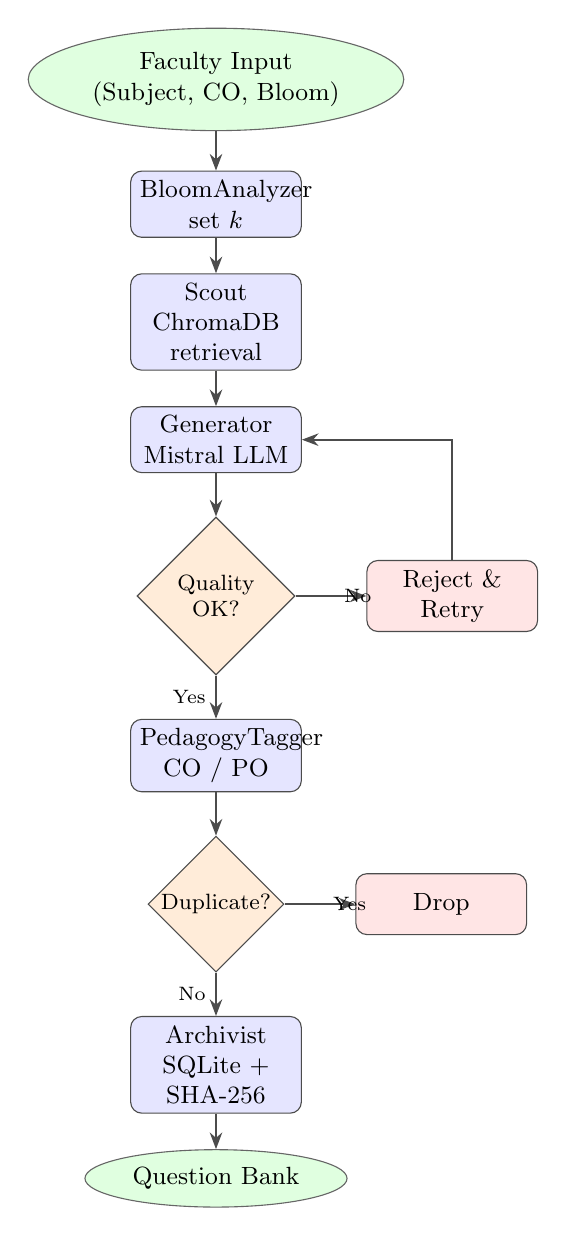
\begin{tikzpicture}[node distance=0.45cm, font=\scriptsize,
    every node/.style={align=center}]

  \node[cloud] (start) {Faculty Input\\(Subject, CO, Bloom)};
  \node[block, below=0.5cm of start] (bloom) {BloomAnalyzer\\set $k$};
  \node[block, below=0.45cm of bloom] (scout) {Scout\\ChromaDB retrieval};
  \node[block, below=0.45cm of scout] (gen2) {Generator\\Mistral LLM};
  \node[decision, below=0.55cm of gen2] (qual) {Quality\\OK?};
  \node[block, right=0.9cm of qual, fill=red!10] (rej) {Reject \&\\Retry};
  \node[block, below=0.55cm of qual] (tag) {PedagogyTagger\\CO / PO};
  \node[decision, below=0.55cm of tag] (dup) {Duplicate?};
  \node[block, right=0.9cm of dup, fill=red!10] (drop) {Drop};
  \node[block, below=0.55cm of dup] (arch) {Archivist\\SQLite + SHA-256};
  \node[cloud, below=0.45cm of arch] (out) {Question Bank};

  \draw[arrow] (start) -- (bloom);
  \draw[arrow] (bloom) -- (scout);
  \draw[arrow] (scout) -- (gen2);
  \draw[arrow] (gen2) -- (qual);
  \draw[arrow] (qual) -- node[right,xshift=1pt]{No} (rej);
  \draw[arrow] (rej) |- (gen2);
  \draw[arrow] (qual) -- node[left]{Yes} (tag);
  \draw[arrow] (tag) -- (dup);
  \draw[arrow] (dup) -- node[right,xshift=1pt]{Yes} (drop);
  \draw[arrow] (dup) -- node[left]{No} (arch);
  \draw[arrow] (arch) -- (out);

\end{tikzpicture}
\caption{Question generation pipeline flowchart. The Scout agent retrieves $k$ chunks from ChromaDB; the Archivist prevents duplicate storage via SHA-256 fingerprinting.}
\label{fig:gen_flow}
\end{figure}

% ─────────────────────────────────────────────────────────────────────────────
\subsection{Module 2: Answer Scheme Parsing}
\label{ssec:scheme}

Faculty upload a PDF answer key. The \texttt{scheme\_parser} module:

\begin{enumerate}
    \item \textbf{Text extraction} — PyMuPDF performs dependency-free direct extraction for typed PDFs. If extracted text is fewer than 50 characters, the engine falls back to pdf2image + EasyOCR for scanned documents.
    \item \textbf{Subject detection} — eight regular-expression patterns match header tokens (\textit{Subject:}, \textit{Course:}, \textit{Paper:}, \textit{Title:}). Filename keywords (\textit{thermodynamics}, \textit{structures}, \textit{propulsion}) serve as a secondary signal.
    \item \textbf{Question segmentation} — eight boundary patterns detect question starts (\texttt{Q1}, \texttt{1.}, \texttt{Question 1}, \texttt{(1)}, etc.). A sequential-number validator rejects spurious matches.
    \item \textbf{Mark extraction} — six patterns parse marks annotations: \texttt{[5M]}, \texttt{(10 marks)}, \texttt{5 marks}, \texttt{M: 5}.
    \item \textbf{Reference answer extraction} — explicit \texttt{Ans:}/\texttt{Sol:} markers, blank-line delimiters, and question-mark detection identify the expected answer text per question.
\end{enumerate}

Parsed structured output (subject, per-question data) is stored as JSON in \texttt{training\_meta.db}.

% ─────────────────────────────────────────────────────────────────────────────
\subsection{Module 3: Answer Script Evaluation Pipeline}
\label{ssec:pipeline}

\subsubsection{OCR Stage}

Student handwritten PDFs are processed by \texttt{ocr\_engine.py}. PyMuPDF is attempted first; if the extracted text is sparse, pdf2image converts each page to a 200 DPI PNG for EasyOCR. Every page yields a confidence score $c_p \in [0, 1]$.

\subsubsection{Answer Segmentation}

A composite regular expression detects question boundaries across the concatenated multi-page text:

\begin{lstlisting}[language=Python, caption={Answer boundary regex}]
_ANSWER_BOUNDARY = re.compile(
  r"(?m)^[\s]*(?:"
  r"(?:ans(?:wer)?\.?\s*)?[Qq](?:uestion)?\.?\s*(\d+)"
  r"|(\d+)[.)]\s"
  r"|(?:ans(?:wer)?\.?\s*(\d+))"
  r")",
)
\end{lstlisting}

Matched segments are mapped to question metadata from the selected answer scheme.

\subsubsection{Type Classification}

Each segment is classified into one of three modalities using weighted keyword signal counting:

\begin{itemize}
    \item \textbf{Theory} — \textit{explain, define, state, differentiate, classify, principle, \ldots}
    \item \textbf{Numerical} — \textit{calculate, determine, stress, strain, moment, efficiency, \ldots}
    \item \textbf{Drawing} — \textit{sketch, draw, diagram, orthographic, cross-section, FBD, \ldots}
\end{itemize}

The modality with the highest signal count is selected.

\subsubsection{OCR Confidence Penalty}

A critical contribution of this work is the \emph{confidence-gated scoring} mechanism. Raw evaluator scores $s_{\text{raw}}$ are attenuated by:

\begin{equation}
    s_{\text{final}} = s_{\text{raw}} \times \min\!\left(1,\; \frac{\bar{c}}{0.70}\right)
    \label{eq:penalty}
\end{equation}

where $\bar{c}$ is the mean per-page OCR confidence for the segment. This prevents semantically similar but orthographically garbled OCR text from inflating cosine-similarity scores. No penalty is applied when $\bar{c} \geq 0.70$.

% ── EVALUATION FLOWCHART ──────────────────────────────────────────────────────
\begin{figure}[H]
\centering
\begin{tikzpicture}[node distance=0.48cm, font=\scriptsize,
    every node/.style={align=center}]

  \node[cloud] (upload) {Student PDF\\Upload};
  \node[block, below=0.5cm of upload] (ocr2) {OCR Engine\\PyMuPDF / EasyOCR};
  \node[block, below=0.45cm of ocr2] (seg) {Segment\\by Q-boundary};
  \node[decision, below=0.55cm of seg] (cls) {Type?};

  \node[block, below left=0.6cm and 0.7cm of cls, fill=indigo!12] (th) {Theory\\Evaluator};
  \node[block, below=0.6cm of cls, fill=amber!15] (nm) {Numerical\\Grader};
  \node[block, below right=0.6cm and 0.7cm of cls, fill=green!12] (dr) {Drawing\\Evaluator};

  \node[block, below=0.6cm of nm, text width=7em] (pen) {OCR Confidence\\Penalty (Eq.~\ref{eq:penalty})};
  \node[block, below=0.5cm of pen] (save) {Persist to\\eval\_results.db};
  \node[cloud, below=0.45cm of save] (rep) {Report +\\Students Page};

  \draw[arrow] (upload) -- (ocr2);
  \draw[arrow] (ocr2) -- (seg);
  \draw[arrow] (seg) -- (cls);
  \draw[arrow] (cls) -| node[above left,xshift=-2pt]{theory} (th);
  \draw[arrow] (cls) -- node[right]{num.} (nm);
  \draw[arrow] (cls) -| node[above right,xshift=2pt]{drawing} (dr);
  \draw[arrow] (th) |- (pen);
  \draw[arrow] (nm) -- (pen);
  \draw[arrow] (dr) |- (pen);
  \draw[arrow] (pen) -- (save);
  \draw[arrow] (save) -- (rep);

\end{tikzpicture}
\caption{Answer script evaluation pipeline. All three modality paths converge at the confidence-penalty stage before result persistence.}
\label{fig:eval_flow}
\end{figure}

% ─────────────────────────────────────────────────────────────────────────────
\subsection{Module 4: Theory Evaluator}
\label{ssec:theory}

Theory answers are scored using a two-signal deterministic blend:

\begin{equation}
    s_{\text{theory}} = \left(\alpha \cdot r_{\text{kw}} + \beta \cdot \text{sim}_{\cos}\right) \times M
    \label{eq:theory}
\end{equation}

where $\alpha = 0.4$, $\beta = 0.6$, $r_{\text{kw}}$ is the fraction of reference keywords present in the student answer (top-15 by TF from the reference), $\text{sim}_{\cos}$ is the cosine similarity between \texttt{all-MiniLM-L6-v2} sentence embeddings of the student and reference answers, and $M$ is the question's maximum marks. Keyword extraction uses a domain-agnostic stopword filter, making the evaluator generalisable to any engineering subject without manual keyword bank curation.

If no reference answer is available (e.g., scheme parsing failed for a question), the system assigns zero and flags the question for mandatory faculty review, avoiding spurious scores from blind semantic comparison.

% ─────────────────────────────────────────────────────────────────────────────
\subsection{Module 5: Numerical Grader}
\label{ssec:numerical}

Numerical answers are evaluated via a step-level rubric executor. When Ollama (Mistral / DeepSeek-R1) is available, chain-of-thought prompting decomposes the student's working into graded steps across five error categories: \textit{formula}, \textit{substitution}, \textit{unit conversion}, \textit{arithmetic}, and \textit{boundary condition}. A heuristic fallback (formula-mention detection + final-answer numeric match) operates when the LLM is unreachable, ensuring graceful degradation.

% ─────────────────────────────────────────────────────────────────────────────
\subsection{Module 6: Drawing Evaluator}
\label{ssec:drawing}

Engineering drawings are inherently spatial and resist purely textual evaluation. Our approach:

\begin{enumerate}
    \item OpenCV preprocessing: CLAHE equalisation $\rightarrow$ Hough-line deskew $\rightarrow$ adaptive thresholding $\rightarrow$ morphological denoising.
    \item EasyOCR extracts text labels and dimension annotations from the processed image.
    \item Extracted tokens are matched against expected parts and dimensions derived from the answer scheme.
    \item Deductions are applied for missing required elements.
    \item All drawing questions are unconditionally flagged for faculty visual review — the AI provides a preliminary label-coverage score only.
\end{enumerate}

% ─────────────────────────────────────────────────────────────────────────────
\subsection{Module 7: Cohen's $\kappa$ Validation}
\label{ssec:kappa}

To quantify evaluator reliability, MechAssess computes Cohen's $\kappa$ between AI scores and faculty-entered reference scores on the same questions:

\begin{equation}
    \kappa = \frac{P_o - P_e}{1 - P_e}
    \label{eq:kappa}
\end{equation}

Scores are discretised into three ordinal buckets — \textit{Low} (0--30\%), \textit{Mid} (31--60\%), \textit{High} (61--100\%) of $M$ — before agreement computation. Faculty scores are entered directly through the Validation Metrics UI and stored in \texttt{kappa\_scores} (within \texttt{eval\_results.db}). Kappa recomputes automatically on each new faculty score entry, removing any reliance on simulated or seeded reference scores.

% ─────────────────────────────────────────────────────────────────────────────
\section{Experimental Evaluation}
\label{sec:eval}

\subsection{Setup}

Experiments were conducted on Aerospace Structures answer scripts submitted by students at RVCE. The answer scheme PDF (\textit{Aerospace\_Structures\_Answer\_Key.pdf}) was uploaded and parsed by the scheme parser. Student handwritten PDFs were evaluated via the \texttt{/api/eval/script} endpoint.

\subsection{Results}

% ── PLACEHOLDER FOR RESULTS FIGURE ──────────────────────────────────────────
\begin{figure}[H]
\centering
% Replace with actual results screenshot / bar chart
\fbox{\parbox{0.9\columnwidth}{\centering\vspace{2cm}
\textbf{[Figure: OCR Confidence vs.\ Score Penalty — insert bar chart here]}\\
\small Plot showing per-page OCR confidence scores alongside raw and penalised evaluation scores across evaluated student scripts.
\vspace{2cm}}}
\caption{Effect of OCR confidence penalty on final scores. Scripts with $\bar{c} < 0.70$ receive attenuated scores, reducing false-positive high marks from garbled OCR text.}
\label{fig:ocr_penalty}
\end{figure}

\begin{figure}[H]
\centering
% Replace with actual kappa results
\fbox{\parbox{0.9\columnwidth}{\centering\vspace{2cm}
\textbf{[Figure: Cohen's $\kappa$ Dashboard — insert screenshot here]}\\
\small Screenshot of the Validation Metrics page showing $\kappa$, per-question AI vs.\ faculty comparison table, and per-type accuracy.
\vspace{2cm}}}
\caption{Cohen's $\kappa$ inter-rater agreement dashboard. Faculty scores entered via the UI are compared against AI scores at bucket level.}
\label{fig:kappa_result}
\end{figure}

\begin{table}[H]
\centering
\caption{Pilot Evaluation Summary (Aerospace Structures)}
\label{tab:results}
\begin{tabular}{lc}
\toprule
\textbf{Metric} & \textbf{Value} \\
\midrule
Scripts evaluated              & \emph{[insert]} \\
Questions per script (avg.)    & \emph{[insert]} \\
Mean OCR confidence            & \emph{[insert \%]} \\
Scripts below confidence threshold ($\bar{c} < 0.70$) & \emph{[insert]} \\
Mean AI score (pre-penalty)    & \emph{[insert / max]} \\
Mean AI score (post-penalty)   & \emph{[insert / max]} \\
Cohen's $\kappa$ (theory)      & \emph{[insert]} \\
Cohen's $\kappa$ (numerical)   & \emph{[insert]} \\
$\kappa$ target ($\geq 0.75$) met & \emph{[Yes / No]} \\
\bottomrule
\end{tabular}
\end{table}

\subsection{Scheme Parsing Accuracy}

The scheme parser successfully extracted question boundaries and marks from typed PDF answer keys in all tested cases. For scanned schemes the EasyOCR fallback achieved adequate extraction when DPI $\geq 200$. Schemes with ambiguous question numbering (e.g., sub-parts labelled \texttt{(a)}, \texttt{(b)}) required the fallback mode, which treats the entire text as a single reference answer.

% ─────────────────────────────────────────────────────────────────────────────
\section{Discussion}
\label{sec:discussion}

\subsection{Key Contributions}

\begin{itemize}
    \item \textbf{Trimodal closed-loop assessment}: To our knowledge, MechAssess is the first open-source system that handles theory, numerical, and drawing modalities within a single evaluation pass triggered by a single file upload.
    \item \textbf{OCR-confidence-gated scoring}: Equation~\eqref{eq:penalty} addresses a critical but often ignored failure mode in OCR-based grading — inflated scores from semantically coherent but orthographically corrupt text.
    \item \textbf{Live $\kappa$ from real scores}: Faculty-entered reference scores replace synthetic proxies, making the inter-rater metric genuinely informative about deployed system reliability.
    \item \textbf{Answer-scheme-driven evaluation}: No per-subject hardcoded keyword banks or rubric databases are required; the system derives all evaluation signals from the uploaded answer scheme.
\end{itemize}

\subsection{Limitations}

\begin{itemize}
    \item EasyOCR accuracy on very light pencil or smudged handwriting is approximately 70--80\%; scanning at $\geq 300$ DPI is strongly recommended.
    \item Drawing evaluation assesses label coverage only — line quality, proportionality, and IS/BIS standard compliance require manual faculty verification.
    \item The scheme parser relies on consistent question numbering; non-standard formats (e.g., unnumbered bullet answers) may not segment correctly.
    \item Numerical LLM grading requires a locally running Ollama instance; the heuristic fallback provides only approximate partial credit.
\end{itemize}

\subsection{Future Work}

\begin{enumerate}
    \item Fine-tune a YOLOv8 model on an annotated corpus of RVCE engineering drawing photographs for geometric element detection beyond label extraction.
    \item Extend the evaluation pipeline to accept student voice responses (speech-to-text $\rightarrow$ theory evaluator) for oral-viva automation.
    \item Integrate CO/PO attainment charts with the live evaluation database, replacing static demo data with question-level CO mappings from the generated question bank.
    \item Conduct a large-scale human-subject study (n $\geq$ 100 scripts, multiple subjects) to establish rigorous $\kappa$ baselines.
\end{enumerate}

% ─────────────────────────────────────────────────────────────────────────────
\section{Conclusion}
\label{sec:conclusion}

We introduced MechAssess, a closed-loop agentic AI assessment platform that unifies question generation and handwritten answer-script evaluation for Mechanical Engineering education. By coupling an eleven-agent LangGraph RAG pipeline with a trimodal OCR-grading backend — governed by faculty-uploaded answer schemes and an OCR-confidence penalty — the system eliminates the principal failure modes of naive LLM-based grading: hallucinated scores, subject-specific brittleness, and unquantified reliability. The replacement of simulated Cohen's $\kappa$ with live faculty-score-based computation closes the validation loop, making system reliability a first-class, continuously monitored quantity rather than a one-time benchmark claim. MechAssess is openly reproducible, runnable on commodity hardware, and designed to grow with real institutional data — making it a credible foundation for AI-augmented assessment practice in Indian technical universities.

% ─────────────────────────────────────────────────────────────────────────────
\section*{Acknowledgment}
The authors thank Dr. Vijayalakshmi M N for her sustained guidance throughout the project. We acknowledge RV College of Engineering for providing computational resources and institutional support. Special thanks to the Mechanical and Aerospace Engineering faculty for providing syllabus materials and reference answer schemes used in evaluation experiments.

% ─────────────────────────────────────────────────────────────────────────────
\begin{thebibliography}{00}

\bibitem{kasneci2023chatgpt}
E. Kasneci et al., ``ChatGPT for good? On opportunities and challenges of large language models for education,'' \textit{Learning and Individual Differences}, vol. 103, p. 102274, 2023.

\bibitem{langgraph2024}
LangChain AI, ``LangGraph: Building Stateful, Multi-Actor Applications with LLMs,'' \url{https://github.com/langchain-ai/langgraph}, 2024.

\bibitem{lindberg2013generating}
A. Lindberg, N. Popowich, J. Nesbit, and P. Winne, ``Generating questions from SQL queries,'' in \textit{Proc. Workshop on Question Generation}, 2013.

\bibitem{heilman2010good}
M. Heilman and N. A. Smith, ``Good question! Statistical ranking for question generation,'' in \textit{Proc. NAACL HLT}, pp. 609--617, 2010.

\bibitem{pan2019recent}
L. Pan, W. Lei, T.-S. Chua, and M. Kan, ``Recent advances in neural question generation,'' \textit{arXiv:1905.08949}, 2019.

\bibitem{burrows2015eras}
S. Burrows, I. Gurevych, and B. Stein, ``The eras and trends of automatic short answer grading,'' \textit{International Journal of Artificial Intelligence in Education}, vol. 25, no. 1, pp. 60--117, 2015.

\bibitem{sultan2016fast}
M. A. Sultan, C. Salazar, and T. Sumner, ``Fast and easy short answer grading with high accuracy,'' in \textit{Proc. NAACL HLT}, pp. 1070--1075, 2016.

\bibitem{guo2022automated}
Q. Guo et al., ``Automated scoring using large language models: A review,'' \textit{arXiv:2212.09562}, 2022.

\bibitem{dzikovska2013semeval}
M. O. Dzikovska et al., ``SemEval-2013 task 7: The joint student response analysis and 8th recognizing textual entailment challenge,'' in \textit{Proc. SemEval}, 2013.

\bibitem{easyocr2020}
J. Baek et al., ``EasyOCR: Ready-to-use OCR with 80+ supported languages,'' \url{https://github.com/JaidedAI/EasyOCR}, 2020.

\bibitem{smith2007overview}
R. Smith, ``An overview of the Tesseract OCR engine,'' in \textit{Proc. ICDAR}, pp. 629--633, 2007.

\bibitem{bluche2016scan}
T. Bluche, J. Louradour, and R. Messina, ``Scan, attend and read: End-to-end handwritten paragraph recognition with MDLSTM attention,'' in \textit{Proc. ICDAR}, pp. 1050--1055, 2017.

\end{thebibliography}

\end{document}
